%\subsection{Service Architecture}

The WMS provides a set of client tools (that will be referred to as WMS-UI from now on) allowing the 
user to access the main services (job management services) made available by the WMS itself. 
These client tools encompass a command line interface, a graphical interface and an API, providing both C$++$ 
and Java bindings, that allow the requests to be submitted and managed programmatically.
In Sections ~\ref{quickstart} and ~\ref{refguide} in particular WMS-UI will indicate the command line interface to the WMS. 

The main operations made possible by the WMS-UI are:
\begin{itemize}
\item Find the list of resources suitable to run a specific job
\item Submit a job/DAG for execution on a remote Computing Element
\item Check the status of a submitted job/DAG	
\item Cancel one or more submitted jobs/DAGs
\item Retrieve the output files of a completed job/DAG (output sandbox)
\item Retrieve and display bookkeeping information about submitted jobs/DAGs
\item Retrieve and display logging information about submitted jobs/DAGs
\item Retrieve checkpoint states of a submitted checkpointable job
\item Start a local listener for an interactive job
\end {itemize}
 
Once submitted from the WMS-UI, the request passes through several other components of the WMS before it 
completes its execution. In such a process the request goes through many states that can be represented 
as a state machine.

The WMS components handling the job are:

\begin{itemize}
\item WMProxy/Network Server 
\item Workload Manager 
\item Resource Broker
\item Job Controller 
\item CondorC/DAGMan
\item Logging and Bookkeeping 
\item Log Monitor 
\end{itemize}


The following picture~\ref{fig-arch} summarizes the internal architecture of the WMS through a package diagram:

\clearpage
\begin{figure}[htb]
\centering
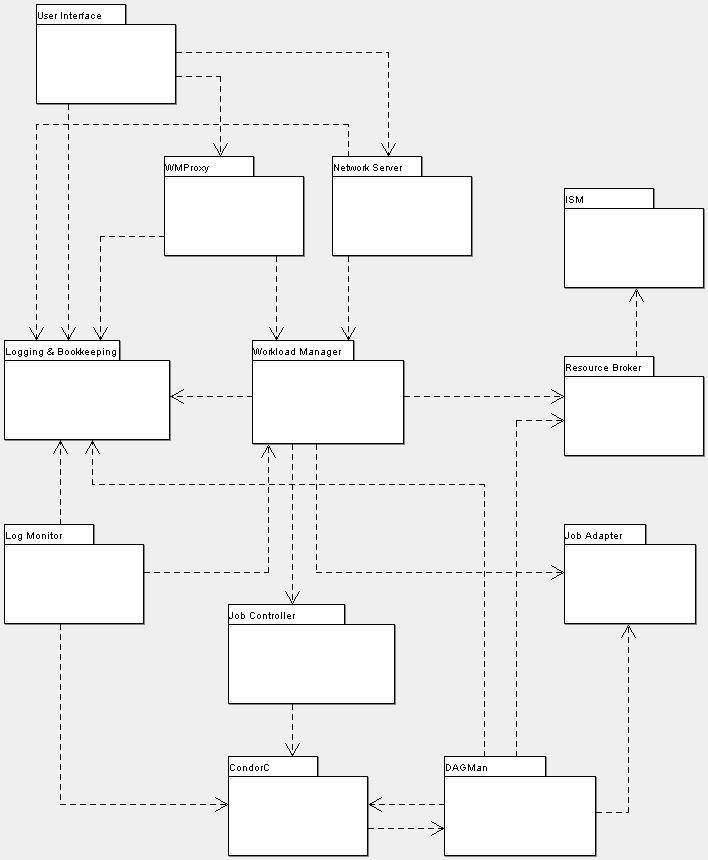
\includegraphics[width=0.92\hsize]{glite-wms}
%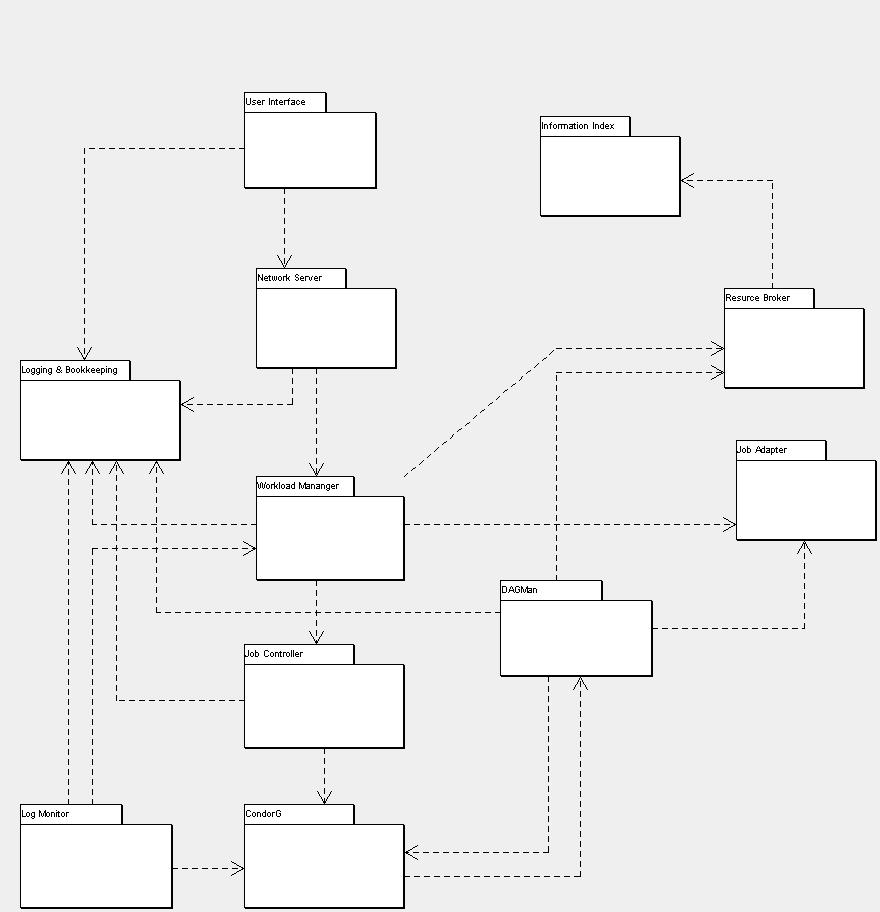
\includegraphics[width=1\hsize]{wp1-arch}
\caption{Overview of the WMS architecture}
\label{fig-arch}
\end{figure}


The {\bf Network Server} (NS) is a generic network daemon that provides support for the job control functionality. 
It is responsible for accepting incoming requests from the WMS-UI (e.g. job submission, job removal), which, if valid, 
are then passed to the Workload Manager.
\medskip

The {\bf Workload Manager Proxy} (WMProxy) is a service providing access to WMS functionality through a Web Services
based interface. Besides being the natural replacement of the NS in the passage to the SOA approach for the WMS 
architecture, it provides additional features such as bulk submission and the support for shared and compressed 
sandboxes for compound jobs. It can be accessed directly through the published WSDL available at 
\url{http://egee-jra1-wm.mi.infn.it/egee-jra1-wm/wmproxy} or using the provided client tools described in ~\cite{WMPROXY}. 

The {\bf Workload Manager} (WM) is the core component of the Workload Management System. Given a valid request, it 
has to take the appropriate actions to satisfy it. To do so, it may need support from other components, which are 
specific to the different request types.

For a computation job there are two main types of request: submission and cancellation. In particular the meaning 
of the submission request is to pass the responsibility of the job to the WM. The WM will then pass the job to an 
appropriate CE for execution, taking into account the requirements and the preferences expressed in the job 
description. The decision of which resource should be used is the outcome of a matchmaking process between the 
submission requests and the available resources. The availability of resources for a particular task depends not 
only on the state of the resources, but also on the utilisation policies that the resource administrators and/or 
the administrator of the VO the user belongs to have put in place.

The {\it Resource Broker} (RB) or Matchmaker is one of the "helper classes" offering support to the WM in 
taking the above mentioned decision. It provides a matchmaking service: given a JDL expression (e.g. for a 
job submission), it finds the resources that best match the request. 

A WM can adopt different policy in order to schedule a job. At one extreme a job is matched to a resource as 
soon as possible and, once the decision has been taken, the job is passed to the selected resource for execution. 
At the other extreme the jobs are held by the WM until a resource becomes available (eager scheduling), at which 
point that resource is matched against the submitted jobs and the job that fits best is passed to the resource 
for immediate execution (lazy scheduling policy). 

The mechanism that allows the flexible application of different policies is the decoupling between the collection 
of information concerning resources and its use.  
The {\it Information Super Market} (ISM) is the component that implements this mechanism and basically consists 
of a repository of resource information that is available in read only mode to the matchmaking engine and whose 
update is the result of either the arrival of notifications or active polling of resources or some arbitrary 
combination of both. Moreover the ISM can be configured so that certain notifications can trigger the matchmaking 
engine. These functionalities besides improving the modularity of the software also support the implementation of 
lazy scheduling policies.

The other fundamental component of the WM internal design is the {\it Task Queue (TQ)}, that gives the possibility 
to keep a submission request for a while if no resources are immediately available that match the job requirements. 
This technique is used, among others, by the AliEn and Condor systems. Non-matching requests will be 
retried either periodically (in an eager scheduling approach) or as soon as notifications of available resources 
appear in the ISM (in a lazy scheduling approach). Alternatively such situations could only lead to an immediate 
abort of the job for lack of a matching resource.
\medskip

Continuing with the WMS components handling the job during its lifetime, we have the {\bf Job Adapter} (JA) which 
is responsible for making the final touches to the JDL expression for a job, before it is passed to CondorC for the 
actual submission. So, besides preparing the CondorC submission file, this module is also responsible for creating 
the job wrapper script that creates the appropriate execution environment in the CE worker node (this includes the 
transfer of the input and of the output sandboxes).
\medskip

{\bf CondorC} is the module responsible for performing the actual job management operations (job submission, 
job removal, etc.), issued on request of the Workload Manager.
\medskip

{\bf DAGMan} (DAG Manager) is a meta-scheduler whose main purpose is to navigate the graph (i.e. the DAG request), 
determine which nodes are free of dependencies, and follow the execution of the corresponding jobs. A DAGMan 
instance is spawned by CondorC for each handled DAG. 

The {\bf Log Monitor} (LM) is responsible for watching the CondorC log file, intercepting interesting events 
concerning active jobs, that is events affecting the job state machine (e.g. job done, job canceled, etc.), and 
therefore triggering appropriate actions.

Moreover a {\bf Proxy Renewal Service} is available to assure that, for all the lifetime of a job, a valid user 
proxy exists within the WMS, and this proxy renewal service relies on the MyProxy service for renewing 
credentials associated to the request.
\medskip

The {\bf Logging and Bookkeeping} (LB) service provides support for the job monitoring functionality: it stores 
logging and bookkeeping information concerning events generated by the various components of the WMS. Using this 
information, the LB service keeps a state machine view of each job.
\medskip

The user can learn in which state its jobs are by querying the LB Service (using the appropriate command provided 
by the WMS-UI). Besides querying for the job state actively, the user may also register for receiving notifications on 
particular job state changes (e.g. when a job terminates). The notifications are delivered using an appropriate 
infrastructure.
